\section{Setup} \label{sec:setup}
There are three different way to get the ROS2 application for the assignment. The first one via git is recommended because it's the fastest one. The others are for simply downloading the zip-folder. 

\subsection{Git}
Navigate into your workspace.
\begin{figure}[H]
    \centering
    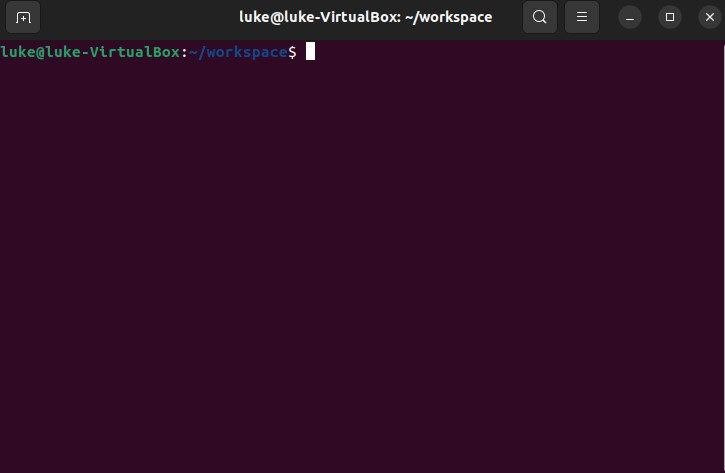
\includegraphics[width=0.8\linewidth]{document//Figure/01workspace.jpg}
    \caption{Workspace}
\end{figure}

Clone the repository. \\ 
\textit{git clone https://github.com/Solaire-42/roboticsAssignment.git}
\begin{figure}[H]
    \centering
    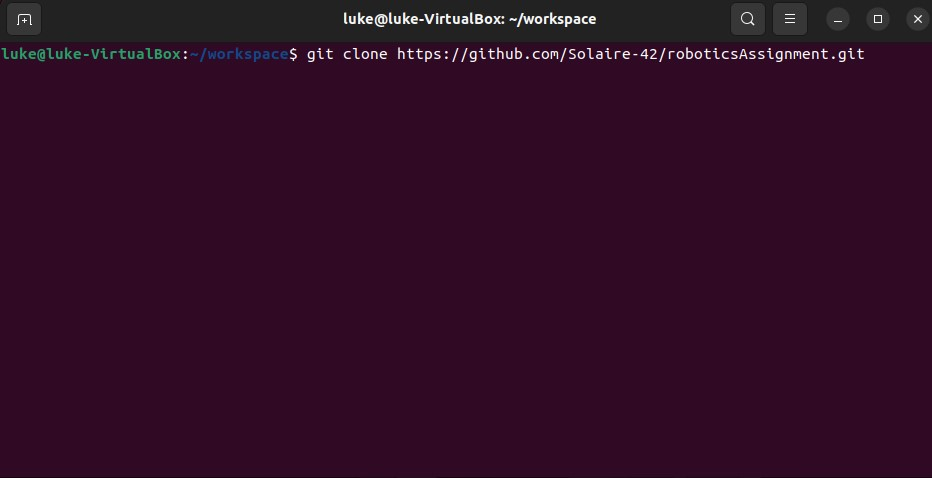
\includegraphics[width=0.8\linewidth]{document//Figure/02clone.jpg}
    \caption{Clone repository}
\end{figure}

\newpage

Navigate into the repository and execute bash file. \\
\textit{cd roboticsAssignment} \\
\textit{bash turtlesimAutomata.sh} \hfill somehow the \textit{sudo bash} command does not work \\
\begin{figure}[H]
    \centering
    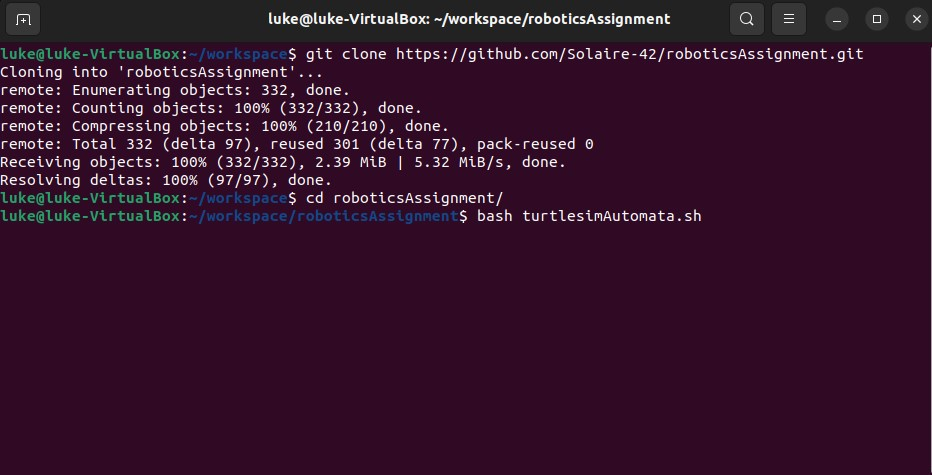
\includegraphics[width=0.8\linewidth]{document//Figure/03execute.jpg}
    \caption{Execute turtlesimAutomata.sh}
\end{figure}

Watch the robot do it's job.
\begin{figure}[H]
    \centering
    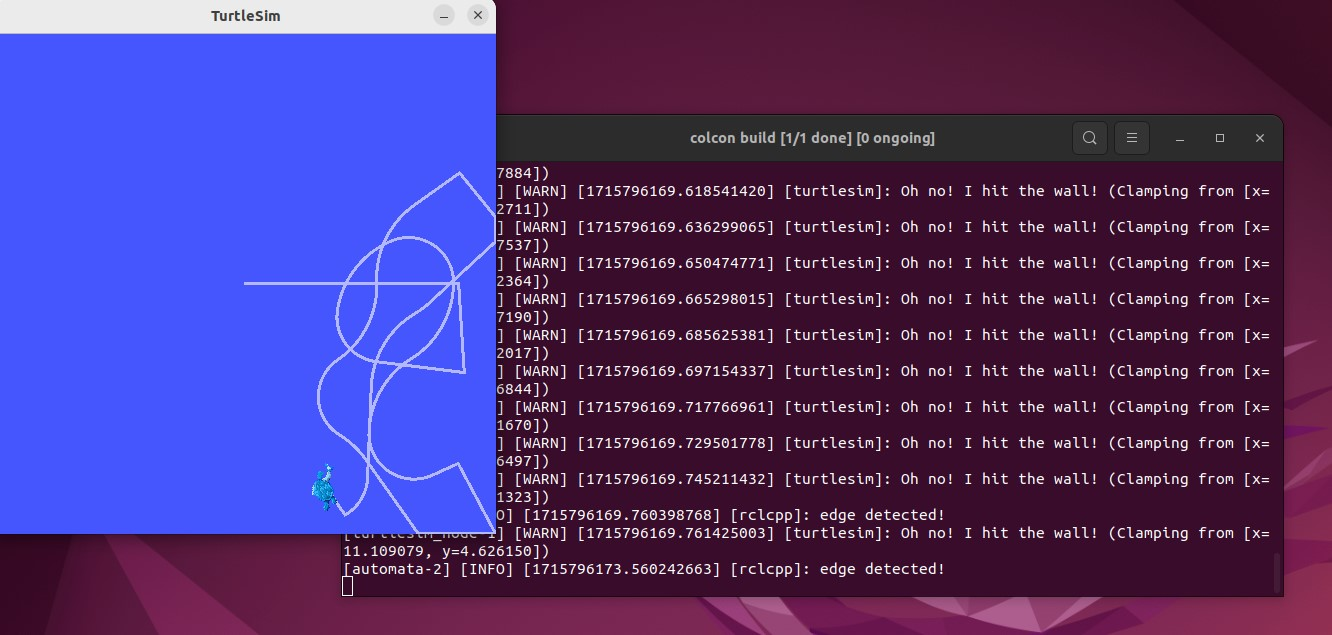
\includegraphics[width=0.8\linewidth]{document//Figure/04turtlesim.jpg}
    \caption{Turtlesim Automata}
\end{figure}

Afterwards the current directory should be empty because the bash script deletes the whole repository before installation in home directory occurs. 

\newpage

\subsection{GitHub Download}
Download zip from GitHub https://github.com/Solaire-42/roboticsAssignment.git.
\begin{figure}[H]
    \centering
    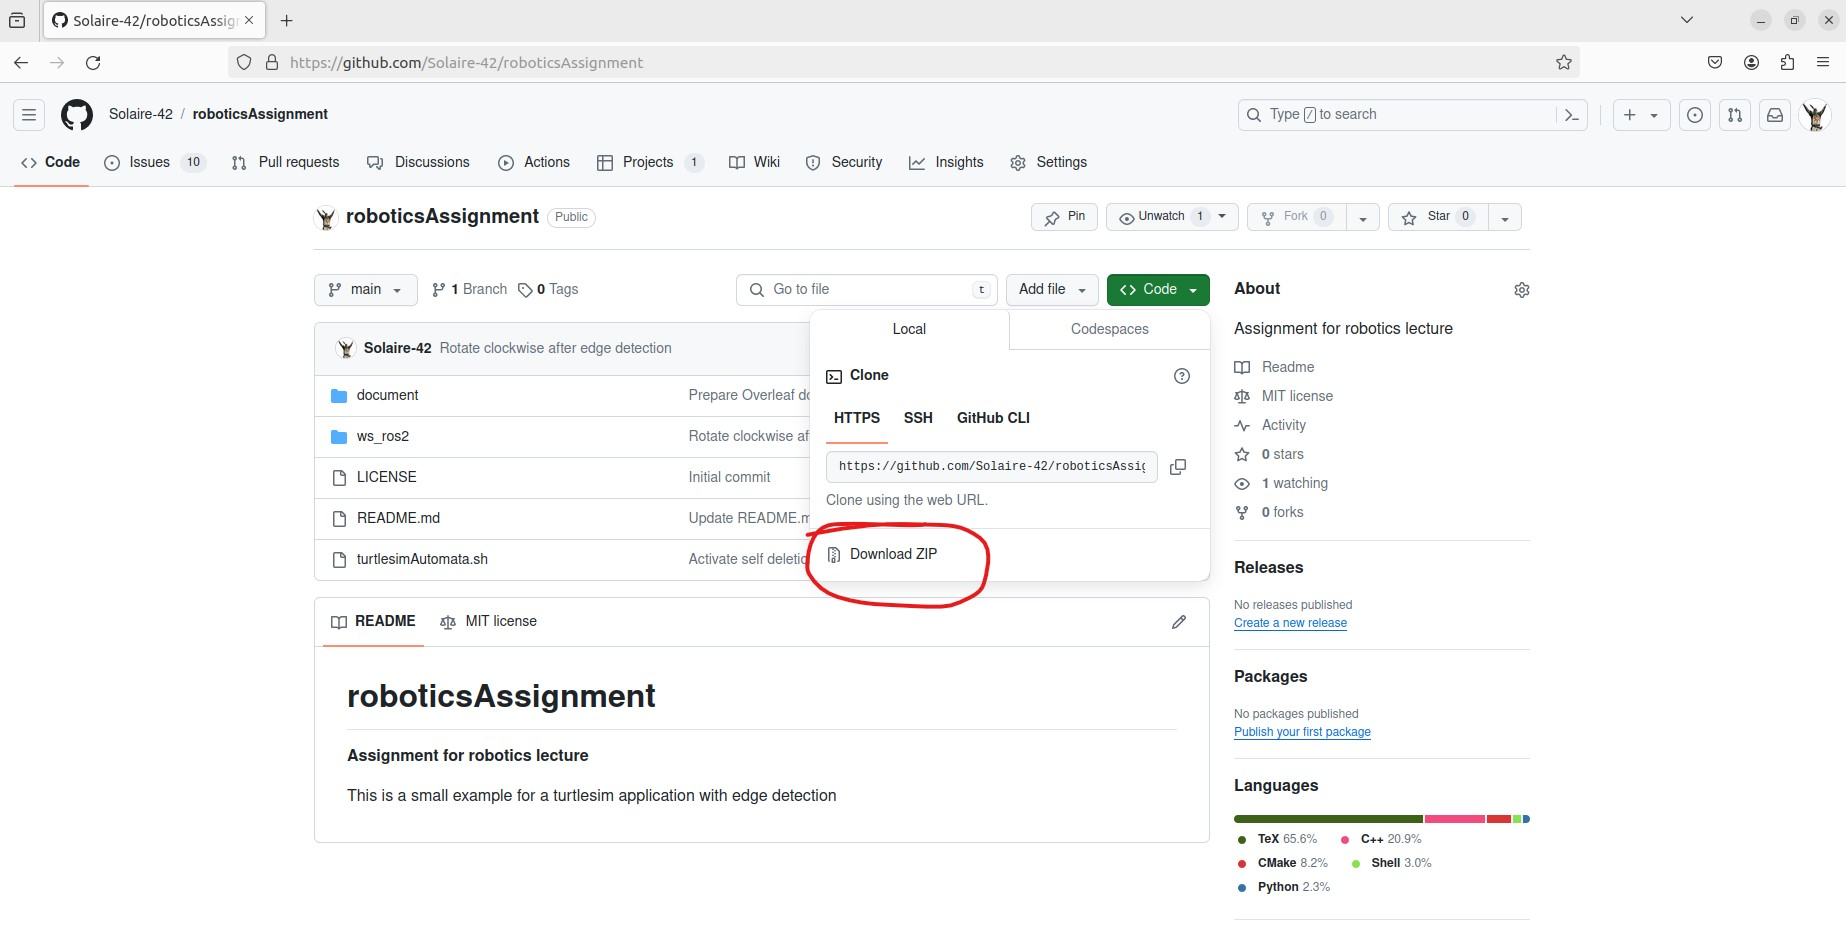
\includegraphics[width=0.8\linewidth]{document//Figure/05download.jpg}
    \caption{GitHub Download}
\end{figure}

Extract here in Downloads folder. 
\begin{figure}[H]
    \centering
    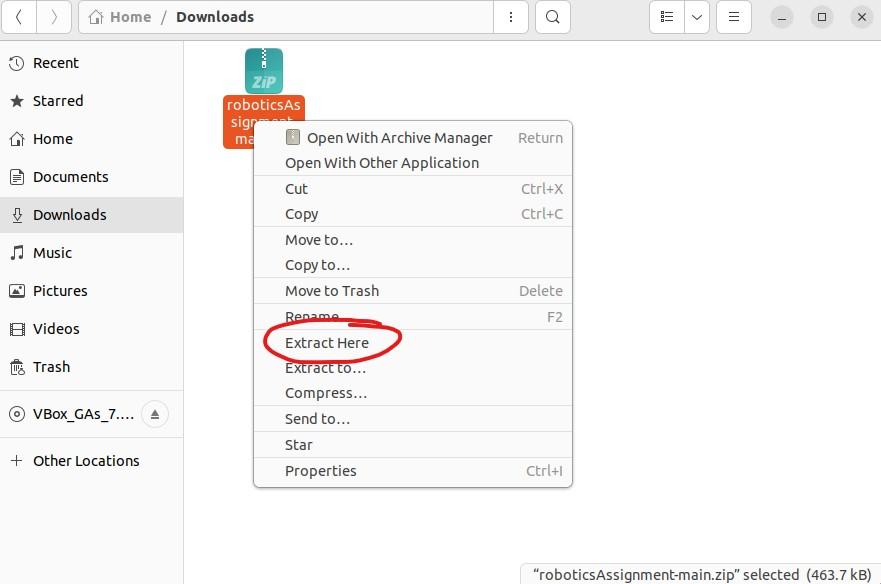
\includegraphics[width=0.8\linewidth]{document//Figure/06extract.jpg}
    \caption{Extract folder}
\end{figure}

Open the folder, open the terminal there and execute bash file.

\newpage

\subsection{Sakai Download}
Download zip from Sakai assignment.

Extract folder and execute bash file. 
